\chapter{Lie Groups: Basic Definitions}
\section{Differential geometry review}
This book assumes that the reader is familiar with basic notions of
differential geometry. For the reader's convenience, in this section, we
briefly remind you of some of the definitions and fix notation for further
use.

Unless otherwise specified, all manifolds considered will be real smooth
manifolds. All manifolds we will consider will have at most countably many
connected components.

For a manifold $M$ and a point $p\in M$, we denote by $T_pM$ the tangent
space to $M$ at point $p$, and by $TM$ the tangent bundle to $M$. The space
of vector fields on $M$ (i.e, global sections of $TM$) is denoted by
$\Vect M$. For a mrphism $f\colon M\to N$ and a point $p\in M$,
$q\coloneq f(p)$, $df\colon T_pM\to T_qN$ is the corresponding map of map
of tangent spaces.

Recall that a morphism $f\colon M\to N$ is called an \emph{immersion} if
$\rk df=\dim M$ for every point $p\in M$; in this case, one can choose
local coordinates in a neighborhood of $p$ and in a neighborhood of $q$
such that $f$ is given by $f(x_1,\dotsc,x_n)=(x_1,\dotsc,x_n,0,\dotsc,0)$.

An \emph{immersed submanifold} in a manifold $M$ is a subset $N\subset M$
with a structure of a manifold (not necessarily the one inherited from $M$)
such that the inclusion map $\iota\colon N\hookrightarrow M$ is an
immersion. Note that the manifold structure on $N$ is part of the data: in
general it is not unique. However, it is usually suppressed in the
notation. Note also that for any point $p\in N$, the tangent space to $N$
is naturally a subspace of the tangent space to $M$ at $p$, i.e.,
$T_pN\subset T_pM$.

An \emph{embedded submanifold $N\subset M$} is an immersed submanifold such
that the inclusion map $\iota\colon N\hookrightarrow M$ is a
homeomorphism. In this case the smooth structure on $N$ is uniquely
determined by the smooth structure on $M$.

Following Spivak, we will use the word submanifold for \emph{embedded
  submanifolds}.

All of the notions above have complex analogs, in which manifolds are
replaced by complex analytic manifolds and smooth maps by holomorphic maps.

\section{Lie groups, subgroups and cosets}
\begin{definition}
  A Lie group is a set $G$ with two structures: $G$ is a group and $G$ is a
  manifold. These structures agree in the following sense: the
  multiplication map $G\times G\to G$ and the inversion map $G\to G$ are
  smooth maps.
\end{definition}

A morphism of Lie groups is a smooth map which also preserves the group
operation: $f(gh)=f(g)f(h)$, $f(1)=1$. We will use the standard notation
$\Img f$ and $\Ker f$ for the image and the kernel of the morphism.

The word real is used to distinguish these Lie groups from complex Lie
groups. However, it is frequently omitted.

One can also consider other classes of manifolds: $C^1$, $C^2$, analytic
(denoted $C^\omega$). It turns out that all of them are equivalent: every
$C^0$ Lie group has a unique analytic structure. This is a higly
non-trivial result (it was one of Hilber's 20 problems), and we are not
going to prove it. Proof of a weaker result, that $C^2$ implies
analyticity, is much easier.

In a similar way, one defines complex Lie groups.

\begin{definition}
  A complex Lie group is a set $G$ with two structures: $G$ is a group and
  $G$ is an analytic manifold. These structures agree in the following
  sense: multiplication map $G\times G\to G$ and inversion map $G\to G$ are
  analytic maps.
\end{definition}

A moprhism of complex Lie groups is an analytic map which also preserves
the group operation, $f(gh)=f(g)f(h)$, $f(1)=1$.

Through out this book, we try to treat both real and complex cases
simultaneously. Thus, most theorems in this book apply both to real and
complex Lie groups.

When talking about complex Lie groups, submanifolds will mean complex
analytic submanifold, tangent spaces will be considered as complex vector
spaces, all morphisms between manifolds will be assumed holomorphic, etc.

\begin{example}
  The following are examples of Lie groups
  \begin{enumerate}[label=(\arabic*)]
  \item $\bbR^n$, with the group operation given by addition
  \item $\bbR^\times\coloneq(\bbR\smallsetminus\{0\},\cdot)$

    $\bbR^+\coloneq(\left\{\,x\in\bbR:x>0\,\right\},+)$
  \item $S^1\coloneq(\left\{\,z\in\bbC:|z|=1\,\right\},\cdot)$
  \item ${\GL_n}\bbR\subset\bbR^{n^2}$. Many of the groups we will consider
    are subgroups of ${\GL_n}\bbR$ or ${\GL_n}\bbC$.
  \item $\SU_2\coloneq\left\{\,A\in\GL_2\bbC:AA^\intercal=I,\det
      A=1\,\right\}$. Indeed, one can easily see that
    \[
      \SU_2=\left\{
        \begin{pmatrix}
          a&b\\
          -\bar b&\bar a
        \end{pmatrix}:
        a,b\in\bbC,\,|a|^2+|b|^2=1\,
      \right\}.
    \]
    Writing $a=x_1+\rmi x_2$, $b=x_3+\rmi x_4$, $x_i\in\bbR$, we see that
    $\SU_2$ is diffeomorphic to
    $S^3=\left\{\,(x_1,x_2,x_3,x_4)\in\bbR^4:{x_1}^2+{x_2}^2+{x_3}^2+{x_4}^2=1\,\right\}$.
  \item In fact, all usual groups of linear algebra, such as ${\GL_n}\bbR$,
    ${\SL_n}\bbR$, $\Orth_n$, $\Unit_n$, $SO_n$, $\SU_n$, $\Sp_{2n}$ are
    all Lie groups.
  \end{enumerate}
\end{example}

Note that this definition of a Lie group does not require $G$ to be
connected. Thus, any finite group is a $0$-dimensional Lie group. Since the
theory of finite groups is complicated enough, it makes sense to separate
the finite part. It can be done as follows.

\begin{theorem}
  Let $G$ be a real or complex Lie group. Denote by $G^0$ the connected
  component of the identity. Then $G^0$ is a normal subgroup of $G$ and is
  a Lie group itself (real or complex, respectively). The quotient group
  $G/G^0$ is discrete.
\end{theorem}
\begin{proof}
We need to show that $G^0$ is closed under the operations of multiplication
and inversion. Since the image of a connected topological space under a
continuous map is connected, the inversion map $i$ must take $G^0$ to one
component of $G$, that which contains $i(1)=1$, namely $G^0$. In a similar
way one shows that $G^0$ is closed under multiplication.

To check that this is a normal subgroup, we must show that if $g\in G$ and
$h\in G^0$, then $ghg^{-1}\in G^0$. Conjugation by $g$ is continuous and
thus will take $G^0$ to some connected component of $G$; since it fixes
$1$, this component is $G^0$.

The fact that the quotient is discrete is obvious.
\end{proof}

This theorem mostly reduces the study of arbitrary Lie groups to the study
of finite groups and connected Lie groups. In fact, one can go further and
reduce the study of connected Lie groups to the study of connected
simply-connected Lie groups.

\begin{theorem}
If $G$ is a connected Lie group, then its universal cover $\tilde G$ has a
canonical structure of a Lie group such that the covering map
$p\colon\tilde G\to G$ is a marphism of a Lie groups whose kernel is
isomorphic to the fundamental group of $G$; $\Ker p=\pi_1(G)$ as a
group. Moreover, in this case $\Ker p$ is a discrete central subgroup in
$\tilde G$.
\end{theorem}
\begin{proof}
The proof follows from the following general result of topology: if $M$,
$N$ are manifolds (or, more generally, nice enough topological spaces),
then any continuous mapping $f\colon M\to N$ can be lifted to a map of
universal covers $\tilde f\colon \tilde M\to\tilde N$. Moreover, if we
choose $m\in M$, $n\in N$ such that $f(m)=n$ and choose liftings $\tilde
m\in M$, $\tilde n\in\tilde N$ such that $p(\tilde m)=m$, $p(\tilde n)=n$,
there is a unique lifting $\tilde f$ of $f$ such that $\tilde f(\tilde
m)=\tilde n$.

Now let us choose some element $\tilde 1\in\tilde G$ such that $p(\tilde
1)=1$ in $G$. Then, by the above theorem, there is a unique map
$\tilde\imath\colon\tilde G\to\tilde G$ which lifts the inversion map
$i\colon G\to G$ and satisfies $\tilde\imath(\tilde 1)=\tilde 1$. In a
similar way, one constructs the multiplication map $\tilde G\times\tilde
G\to\tilde G$.

Finally, the fact that $\Ker p$ is central follows from the results of
Exercise 2.2. (Whatever that exercise may be.)
\end{proof}

\begin{definition}
A closed Lie subgroup $H$ of a Lie group $G$ is a subgroup which is also a
submanifold.
\end{definition}

\begin{theorem}
  \begin{enumerate}[label=\textnormal{(\arabic*)}]
  \item Any closed LIe subgroup is closed in $G$.
  \item Any closed subgroup of a Lie goup is a closed real Lie subgroup.
  \end{enumerate}
\end{theorem}
\begin{proof}
The proof o fthe first part is given in Exercise 2.1. The second part is
much harder and will not be proved here. Thep roof uses the technique of
Lie algebras and can be found, for example, in 10, Corollary 1.10.7.
\end{proof}

\begin{corollary}
  \hfill
  \begin{enumerate}[label=\textnormal{(\arabic*)}]
  \item If $G$ is a connected LIe group and $U$ is a neighborhood of $1$,
    then $U$ generates $G$.
  \item Let $f\colon G_1\to G_2$ be a morphism of Lie groups, with $G_2$
    connected, such that $df\colon T_1G_1\to T_2G_2$ is surjective. Then
    $f$ is surjective.
  \end{enumerate}
\end{corollary}
\begin{proof}
(1) Let $H$ be the subgroup generated by $U$. Then $H$ is open in $G$: for
any element $h\in H$, the set $h\cdot U$ is a neighborhoof of $h$ in
$G$. Since it is an open subset of a manifold, it is a submanifold, so $H$
is a closed Lie subgroup. Therefore, by Theorem 2.9 it is closed and is
nonempty, so $H=G$.
\\\\
(2) Given the assumptions, the inverse function theorem says that $f$ is
surjective onto some neighborhood $U$ of $1\in G_2$. Since an image of
a group morphism is a subgroup, and $U$ generates $G_2$, $f$ is
surjective.
\end{proof}

As in the theory of discrete groups, given a closed Lie subgroup $H<G$, we
can define the notion of cosets and define the coset space $G/H$ as the set
of equivalence classes. The following theorem shows that the coset space is
actually a manifold.
\begin{theorem}
  \hfill
  \begin{enumerate}[label=\textnormal{(\arabic*)}]
  \item Let $G$ be a Lie group of dimension $n$ and $H<G$ a closed Lie
    subgroup of dimension $k$. Then the coset space $G/H$ has a natural
    structure of a manifold of dimension $n-k$ such that the canonical map
    $p\colon G\to G/H$ is a fiber bundle, with fiber diffeomorphic to
    $H$. The tangent space at $\tilde 1=p(1)$ is given by $T_{\tilde
      1}G/H=T_1G/T_1H$.
  \item If $H$ is a normal closed Lie subgroup then $G/H$ has a canonical
    structure of a Lie group.
  \end{enumerate}
\end{theorem}
\begin{proof}
  Denote by $p\colon G\to G/H$ the canonical map. Let $g\in G$ and
  $\bar g=p(g)\in G/H$. Then the set $g\cdot H$ is a submanifold in $G$ as
  it is an image of $H$ under diffeomorphism $x\mapsto gx$. Choose a
  submanifold $M\subset G$ such that $g\in M$ and $M$ is transversal to the
  manifold $gH$, i.e., $T_gG=T_ggH\oplus T_gM$. Let $U\subset M$ be a
  sufficiently small neighborhood of $g$ in $M$. Then the set
  $UH\coloneq\left\{\,uh:u\in U,h\in H\,\right\}$ is open in $G$ (which
  easily follows from the inverse function theorem applied to the map
  $U\times H\to G$). Consider $\bar U=p(U)$; since $p^{-1}(\bar U)=UH$ is
  open, $\bar U$ is an open neighborhood of $\bar g$ in $G/H$ and the map
  $U\to \bar U$ is a homeomorphism. This gives a local chart for $G/H$ and
  at the same time shows that $G\to G/H$ is a fiber bundle with fiber
  $H$. Now we just need to show that the transition functions between such
  charts are smooth and that the smooth structure does not depend on the
  choice of $g$, $M$.

  This argument also shows that the kernel of the projection $\pi\colon
  T_gG\to T_{\bar g}G/H$ is equal to $T_ggH$. In particular, for $g=1$ this
  gives us an isomorphism $T_{\bar 1}G/H\simeq T_1G/T_1H$.
\end{proof}

\begin{corollary}
  Let $H$ be a closed Lie subgroup of a Lie group $G$.
  \begin{enumerate}[label=\textnormal{(\arabic*)}]
  \item If $H$ is connected, then the set of connected components
    $\pi_0G=\pi_0G/H$ . In particular, if $H$, $G/H$ are connected, then so
    is $G$.
  \item If $G$, $H$ are connected, then there is an exact sequence of
    fundamental groups
    \[
      \pi_2G/H\longrightarrow
      \pi_1H\longrightarrow
      \pi_1G/H\longrightarrow
      1.
    \]
  \end{enumerate}
\end{corollary}
This corollary follows from more general long exact sequence of homotopy
groups associated with any fiber bundle.

\section{Analytic subgroups and the homomorphism theorem}
For many purposes, the notion of a closed Lie subgroup introduced above is
too restrictive. For example
\begin{example}
Let $G_1\coloneq\bbR$, $G_2\coloneq T^2=\bbR^2/\bbZ^2$. Define the map
$f\colon G_1\to G_2$ by $f(t)\coloneq(t\mod\bbZ,\alpha t\mod\bbZ)$, where
$\alpha$ is some fixed irrational number. Then it is well-known that the
image of this map is everywhere dense in $T^2$ (it is sometimes called the
\emph{irrational winding} on the torus)..
\end{example}

It is therefore useful to introduce a more general notion of a
subgroup. Recall the definition of immersed submanifold.

\begin{definition}
  A \emph{Lie subgroup} in a Lie  group $H<G$ is an immersed submanifold
  which is also a subgroup.
\end{definition}

It is easy to see that in such a situation $H$ is itself a Lie group and
the inclusion map $\iota\colon H\hookrightarrow G$ is a morphism of Lie
groups.

Clearly, every closed Lie subgroup is a Lie subgroup, but the converse is
not true as the example above demonstrated.

With this new notion of a subgroup we can formulate an analog of the
standard homomorphism theorems.

\begin{theorem}
Let $f\colon G_1\to G_2$ be a morphism of Lie groups. Then $H\coloneq\Ker
f$ is a normal closed Lie subgroup in $G_1$, and $f$ gives rise to an
injective morphism $G_1/H\to G_2$, which is an immersion; thus, $\Img f$ is
a Lie subgroup in $G_2$. If $\Img f$ is a submanifold, then it is a closed
lie subgroup in $G_2$ and $f$ gives an isomorphism of Lie gruops
$G_1/H\simeq\Img f$.
\end{theorem}

With this new notation of of a subgroup we can formulate an analog of the
standard hobmomorphism theorems.
\begin{theorem}
  Let $f\colon G_1\to G_2$ be a morphism of Lie groups. Then
  $H\coloneq\Ker f$ is a normal closed Lie subgroup in $G_1$, and $f$ gives
  rise to an injective morphism $G_1/H\to G_2$, which is an immersion;
  thus, $\Img f$ is a Lie subgroup of $G_2$. If $\Img f$ is a submanifold
  then it is a closed Lie subgroup in $G_2$ and $f$ gives an isomorphism of
  Lie groups $G_1/H\simeq\Img f$.
\end{theorem}

The easiest way to prove this theorem is by using the theory of Lie
algebras which we develeop in the next chapter.

\section{Action of Lie groups on manifolds and representations}
The primary reason why Lie groups are so frequently used is that they
usually appear as symmetry groups of various geometric objects. In this
section, we will show several examples.

\begin{definition}
  An action of a real Lie group $G$ on a manifold $M$ is an assignment to
  each $g\in G$ of a diffeomorphism $\rho(g)\in\Diff M$ such that
  $\rho(1)=\id$, $\rho(gh)=\rho(g)\rho(h)$ and such that the map
  \[
    \begin{aligned}
      G\times M&\longrightarrow M\\
      (g,m)&\longmapsto \rho(g)m
    \end{aligned}
  \]
  is a smooth map.
\end{definition}

A holomorphic action of a complex Lie group $G$ on a complex manifold $M$
is an assignment to each $g\in G$ an invertible holomorphic map
$\rho(g)\in\Diff M$ such that $\rho(1)=\id$, $\rho(gh)=\rho(g)\rho(h)$ and
such that the map
\[
  \begin{aligned}
    G\times M&\longrightarrow M\\
    (g,m)&\longmapsto \rho(g)m
  \end{aligned}
\]
is holomorphic.

\begin{example}
  \hfill
  \begin{enumerate}[label=(\arabic*)]
  \item The group ${\GL_n}\bbR$ acts on $\bbR^n$.
  \item The group $\Orth_n$ acts on the sphere $S^{n-1}\subset\bbR^n$. The
    group $\Unit_n$ acts on the sphere $S^{2n-1}\subset\bbC^n$.
  \end{enumerate}
\end{example}
Closely related with the notion of a group action on a manifold is the
notion of a representation.

\begin{definition}
A representation of a Lie group $G$ is a vector space $V$ together with a
group morphism $\rho\colon G\to\End V$. If $V$ is finite-dimensional, we
require that $\rho$ be smooth (respectively, analytic), so it is a morphism
of Lie groups. A morphism between two representations $V$, $W$ of the same
group $G$ is a linear map $f\colon V\to W$ which commutes with the group
action: $f\circ\rho_v(g)=\rho_w(g)\circ f$.
\end{definition}

In other words, we assigne to every $g\in G$ a linear map $\rho(g)\colon
V\to V$ so that $\rho(g)\rho(h)=\rho(gh)$.

We will frequently use the shorter notation $g\cdot m$, $g\cdot v$ instead
of $\rho(g)(m)$ in the cases where there is no ambiguity about the
representation being used.

Any action of the group $G$ on a manifold $M$ gives rise to several
representations of $G$ on various vector spaces associated with $M$:
\begin{enumerate}[label=(\arabic*)]
\item Representation of $G$ on the infinite-dimensional space of functions
  $C^\infty(M)$ or the space of holomorphic functions $C^\omega(M)$ defined
  by
  \[
    (\rho(g)\circ f)(m)\coloneq f(g^{-1}\cdot m).
  \]
  (note that we need $g^{-1}$ rather than $g$ to satisfy
  $\rho(g)\rho(h)=\rho(gh)$).
\item Representation of $G$ on the infinite-dimensional space of vector
  fields $\Vec M$ defined by
  \[
    (\rho(g)(\bfv))(m)\coloneq dg(\bfv(g^{-1}\cdot m)).
  \]
  In a similar way, we defined the action of $G$ on the spaces of
  differential forms and other types of tensor fields on $M$.
\item Assume that $m\in M$ is a fixed-point: $g\cdot m=m$ for all $g\in
  G$. Then we have an action of $G$ on the tangent space $T_mM$ given by
  $\rho(g)=dg\colon T_mM\to T_mM$, and similarly for the spaces $T_m^*M$,
  $\bigwedge^k T_m^*M$.
\end{enumerate}

\section{Orbits and homogeneous spaces}
Let $G$ be a Lie group acting on a manifold $M$. Then for every point
$m\in M$ we defined its \emph{orbit} by
$\calO_m\coloneq Gm\coloneq\left\{\,g\cdot m:g\in G\,\right\}$ and
stabilizer
\[
G_m\coloneq\left\{\,g\in G:g\cdot m=m\,\right\}.
\]

\begin{theorem}
  Let $M$ be a manifold with an action of a Lie group $G$. Then for any
  $m\in M$ the stabilizer $G_m$ is closed is a closed Lie subgroup in $G$,
  and $g\mapsto g\cdot m$ is an injective immersion $G/G_m\hookrightarrow
  M$ whose image coincides with the orbit $\calO_m$.
\end{theorem}

\begin{proof}
  The fact that the orbit is in bijection with $G/G_m$ is obvious. For the
  proof of the fact that $G_m$ is a closed Lie subgroup, we could just
  refer to Theorem 2.9. However, this would not help proving that
  $G/G_m\to M$ is an immersion. Both of these statements are esiest proved
  using the technique of Lie algebras.
\end{proof}

\begin{corollary}
  The orbit $\calO_m$ is an immersed submanifold in $M$, with tangeth space
  $T_m\calO_m\simeq T_1G/T_1G_m$. If $\calO_m$ is a submanifold, then
  $g\mapsto g\cdot m$ is a diffeomorphism $G/G_m\rightleftarrows\calO_m$.
\end{corollary}

An important special case is when the action of $G$ is transitive, i.e.,
when there is only one orbit.

\begin{definition}
  A $G$-homogeneous space is a manifold with a transitive action of $G$.
\end{definition}

As an immediate corollary of Corollary 2.21, we see that each homogeneous
space is diffeomorphic to a coset space $G/H$. Combining Theorem 2.11, we
get the following result.

\begin{corollary}
  Let $M$ be a $G$-homogeneous space and choose $m\in M$. Then the map
  $G\to M$ given by $g\mapsto g\cdot m$ is a fiber bundle over $M$ with
  fiber $G_m$.
\end{corollary}

\begin{enumerate}[label=(\arabic*)]
\item Consider the action of $\SO_n\bbR$ on the sphere
  $S^{n-1}\subset\bbR^n$. It is transitive then $S^{n-1}$ is a homogeneous
  space, so we have the fiber bundle
  \[
    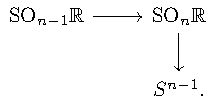
\includegraphics{fiber-bundle-so}
  \]
\item Consider the action of $\SU_n$ on the sphere
  $S^{2n-1}\subset\bbC^n$. Then it is a homogeneous space, so we have a
  fiber bundle
  \[
    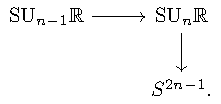
\includegraphics{fiber-bundle-su}
  \]
\end{enumerate}

In fact, action of $G$ can be used to define smooth structure on a
set. Indeed, if $M$ is a set (with no predetermined smooth structure) with
a transitive action of a Lie group $G$, then $M$ is in bijection with
$G/H$, $H\coloneq\Stab_G m$ and thus, by Theorem 2.11 $M$ has a canonical
structure of a manifold of dimension $\dim G-\dim H$.

\begin{example}
  Define a \emph{flag} in $\bbR^n$ to be a sequence of subspaces
  \[
    \{0\}\subset V_1\subset V_2\subset\dotsb\subset V_n=\bbR^n,\qquad \dim
    V_i=i.
  \]
  Let $\calF_n(\bbR)$ be the set of all flags in $\bbR^n$. It turns out
  that $\calF_n(\bbR)$ has a canonical structure of a smooth manifold which
  is called the \emph{flag manifold}. The easiest way to define it is to
  note that we have an obvious action of the group ${\GL_n}\bbR$ on
  $\calF_n(\bbR)$. This action is transitive: by a change of basis, any
  flag can be identified with the standard flag
  \[
    V^{\text{std}}\coloneq\left( \{0\}\subset\Span(\bfe_1
      )\subset\Span(\bfe_1,\bfe_2
      )\subset\cdots\subset\Span(\bfe_1,\dotsc,\bfe_n )=\bbR\right)
  \]
  where $\langle \bfe_1,\dots,\bfe_n \rangle$ is the standard basis for
  $\bbR^n$. Thus, $\calF_n(\bbR)$ can be identified with the coset space
  ${\GL_n}\bbR/B_n\bbR$ where $B_n\bbR\coloneq\Stab V^{\text{std}}$ is the
  group of all invertible upper-triangular matrices. Therefore, $\calF_n$
  is a manifold of dimension $n^2-n(n+1)/2=n(n-1)/2$.
\end{example}

%%% Local Variables:
%%% mode: latex
%%% TeX-master: "../MA598-Lie-Groups"
%%% End:
